%----------------------------------------------------------------------------------------
%	PACKAGES AND OTHER DOCUMENT CONFIGURATIONS
%----------------------------------------------------------------------------------------

\documentclass{article}
\renewcommand{\baselinestretch}{1.5} 
\usepackage[T1]{fontenc}
\usepackage{graphicx}
\usepackage{caption}
\captionsetup[figure]{
    position=above,font=large,labelfont=large
}

%%%%%%%%%%%%%%%%%%%%%%%%%%%%%%%%%%%%%%%%%
% Lachaise Assignment
% Structure Specification File
% Version 1.0 (26/6/2018)
%
% This template originates from:
% http://www.LaTeXTemplates.com
%
% Authors:
% Marion Lachaise & François Févotte
% Vel (vel@LaTeXTemplates.com)
%
% License:
% CC BY-NC-SA 3.0 (http://creativecommons.org/licenses/by-nc-sa/3.0/)
% 
%%%%%%%%%%%%%%%%%%%%%%%%%%%%%%%%%%%%%%%%%

%----------------------------------------------------------------------------------------
%	PACKAGES AND OTHER DOCUMENT CONFIGURATIONS
%----------------------------------------------------------------------------------------

\usepackage{amsmath,amsfonts,stmaryrd,amssymb} % Math packages

\usepackage{enumerate} % Custom item numbers for enumerations

\usepackage[ruled]{algorithm2e} % Algorithms

\usepackage[framemethod=tikz]{mdframed} % Allows defining custom boxed/framed environments

\usepackage{listings} % File listings, with syntax highlighting
\lstset{
	basicstyle=\ttfamily, % Typeset listings in monospace font
}

%----------------------------------------------------------------------------------------
%	DOCUMENT MARGINS
%----------------------------------------------------------------------------------------

\usepackage{geometry} % Required for adjusting page dimensions and margins

\geometry{
	paper=a4paper, % Paper size, change to letterpaper for US letter size
	top=2.5cm, % Top margin
	bottom=3cm, % Bottom margin
	left=2.5cm, % Left margin
	right=2.5cm, % Right margin
	headheight=14pt, % Header height
	footskip=1.5cm, % Space from the bottom margin to the baseline of the footer
	headsep=1.2cm, % Space from the top margin to the baseline of the header
	%showframe, % Uncomment to show how the type block is set on the page
}

%----------------------------------------------------------------------------------------
%	FONTS
%----------------------------------------------------------------------------------------

\usepackage[utf8]{inputenc} % Required for inputting international characters
\usepackage[T1]{fontenc} % Output font encoding for international characters

\usepackage{XCharter} % Use the XCharter fonts

%----------------------------------------------------------------------------------------
%	COMMAND LINE ENVIRONMENT
%----------------------------------------------------------------------------------------

% Usage:
% \begin{commandline}
%	\begin{verbatim}
%		$ ls
%		
%		Applications	Desktop	...
%	\end{verbatim}
% \end{commandline}

\mdfdefinestyle{commandline}{
	leftmargin=10pt,
	rightmargin=10pt,
	innerleftmargin=15pt,
	middlelinecolor=black!50!white,
	middlelinewidth=2pt,
	frametitlerule=false,
	backgroundcolor=black!5!white,
	frametitle={Command Line},
	frametitlefont={\normalfont\sffamily\color{white}\hspace{-1em}},
	frametitlebackgroundcolor=black!50!white,
	nobreak,
}

% Define a custom environment for command-line snapshots
\newenvironment{commandline}{
	\medskip
	\begin{mdframed}[style=commandline]
}{
	\end{mdframed}
	\medskip
}

%----------------------------------------------------------------------------------------
%	FILE CONTENTS ENVIRONMENT
%----------------------------------------------------------------------------------------

% Usage:
% \begin{file}[optional filename, defaults to "File"]
%	File contents, for example, with a listings environment
% \end{file}

\mdfdefinestyle{file}{
	innertopmargin=1.6\baselineskip,
	innerbottommargin=0.8\baselineskip,
	topline=false, bottomline=false,
	leftline=false, rightline=false,
	leftmargin=2cm,
	rightmargin=2cm,
	singleextra={%
		\draw[fill=black!10!white](P)++(0,-1.2em)rectangle(P-|O);
		\node[anchor=north west]
		at(P-|O){\ttfamily\mdfilename};
		%
		\def\l{3em}
		\draw(O-|P)++(-\l,0)--++(\l,\l)--(P)--(P-|O)--(O)--cycle;
		\draw(O-|P)++(-\l,0)--++(0,\l)--++(\l,0);
	},
	nobreak,
}

% Define a custom environment for file contents
\newenvironment{file}[1][File]{ % Set the default filename to "File"
	\medskip
	\newcommand{\mdfilename}{#1}
	\begin{mdframed}[style=file]
}{
	\end{mdframed}
	\medskip
}

%----------------------------------------------------------------------------------------
%	NUMBERED QUESTIONS ENVIRONMENT
%----------------------------------------------------------------------------------------

% Usage:
% \begin{question}[optional title]
%	Question contents
% \end{question}

\mdfdefinestyle{question}{
	innertopmargin=1.2\baselineskip,
	innerbottommargin=0.8\baselineskip,
	roundcorner=5pt,
	nobreak,
	singleextra={%
		\draw(P-|O)node[xshift=1em,anchor=west,fill=white,draw,rounded corners=5pt]{%
		Question \theQuestion\questionTitle};
	},
}

\newcounter{Question} % Stores the current question number that gets iterated with each new question

% Define a custom environment for numbered questions
\newenvironment{question}[1][\unskip]{
	\bigskip
	\stepcounter{Question}
	\newcommand{\questionTitle}{~#1}
	\begin{mdframed}[style=question]
}{
	\end{mdframed}
	\medskip
}

%----------------------------------------------------------------------------------------
%	WARNING TEXT ENVIRONMENT
%----------------------------------------------------------------------------------------

% Usage:
% \begin{warn}[optional title, defaults to "Warning:"]
%	Contents
% \end{warn}

\mdfdefinestyle{warning}{
	topline=false, bottomline=false,
	leftline=false, rightline=false,
	nobreak,
	singleextra={%
		\draw(P-|O)++(-0.5em,0)node(tmp1){};
		\draw(P-|O)++(0.5em,0)node(tmp2){};
		\fill[black,rotate around={45:(P-|O)}](tmp1)rectangle(tmp2);
		\node at(P-|O){\color{white}\scriptsize\bf !};
		\draw[very thick](P-|O)++(0,-1em)--(O);%--(O-|P);
	}
}

% Define a custom environment for warning text
\newenvironment{warn}[1][Warning:]{ % Set the default warning to "Warning:"
	\medskip
	\begin{mdframed}[style=warning]
		\noindent{\textbf{#1}}
}{
	\end{mdframed}
}

%----------------------------------------------------------------------------------------
%	INFORMATION ENVIRONMENT
%----------------------------------------------------------------------------------------

% Usage:
% \begin{info}[optional title, defaults to "Info:"]
% 	contents
% 	\end{info}

\mdfdefinestyle{info}{%
	topline=false, bottomline=false,
	leftline=false, rightline=false,
	nobreak,
	singleextra={%
		\fill[black](P-|O)circle[radius=0.4em];
		\node at(P-|O){\color{white}\scriptsize\bf i};
		\draw[very thick](P-|O)++(0,-0.8em)--(O);%--(O-|P);
	}
}

% Define a custom environment for information
\newenvironment{info}[1][Info:]{ % Set the default title to "Info:"
	\medskip
	\begin{mdframed}[style=info]
		\noindent{\textbf{#1}}
}{
	\end{mdframed}
}
 % Include the file specifying the document structure and custom commands

%----------------------------------------------------------------------------------------
%	ASSIGNMENT INFORMATION
%----------------------------------------------------------------------------------------

\title{Project - Database Security} % Title of the assignment

\author{Ciprian-Mihai Ceausescu\\ \texttt{ciprian-mihai.ceausescu@my.fmi.unibuc.ro}} % Author name and email address

\date{University of Bucharest --- \today} % University, school and/or department name(s) and a date

%----------------------------------------------------------------------------------------

\begin{document}

\maketitle % Print the title

%----------------------------------------------------------------------------------------
%	Introduction
%----------------------------------------------------------------------------------------

\section*{Introduction}
\hspace{10mm}In this project is presented a database model for a company that can sells \textbf{products} to \textbf{users} and, also, saves a history of all \textbf{orders}. The entities are the following:
\begin{itemize}
\item user -  the main entity contains the following information: \textbf{authentication} e-mail, password, reset password token and timestamp, created and updated timestamps.
\item role - contains the following information: \textbf{name} of the role, created and updated timestamps.
\item product -  contains the following information: \textbf{name} of the product, description, price, image url, created and updated timestamps.
\item order - contains the following information: \textbf{pay type}, how the product is delivered, created and updated timestamps.
\end{itemize}
%----------------------------------------------------------------------------------------
%	Main database diagram
%----------------------------------------------------------------------------------------
\begin{figure}
\centering
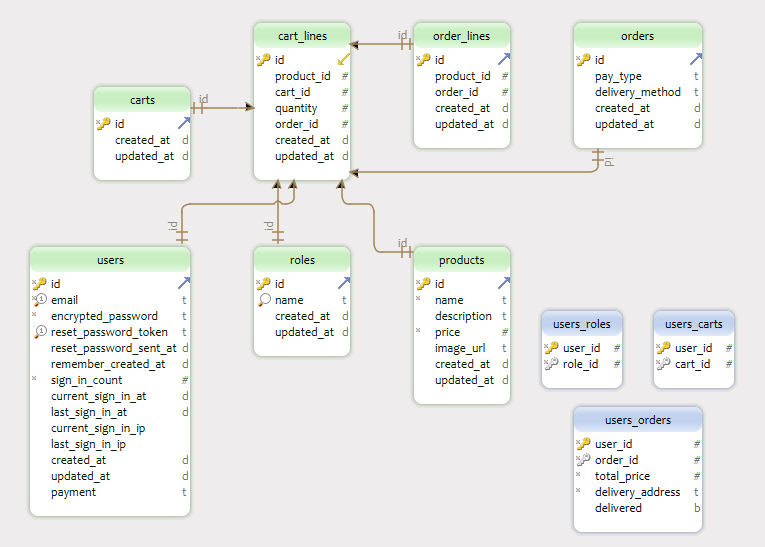
\includegraphics[scale=0.8]{Schema_1}
\caption{Main database diagram}
\end{figure}
%----------------------------------------------------------------------------------------
%	Audit database diagram
%----------------------------------------------------------------------------------------
\begin{figure}
\centering
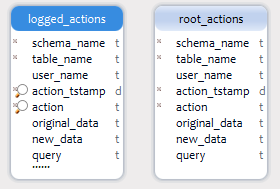
\includegraphics[scale=1]{Schema_2}
\caption{Audit database diagram}
\end{figure}
%----------------------------------------------------------------------------------------
%	Database and tables
%----------------------------------------------------------------------------------------
\begin{figure}
\centering
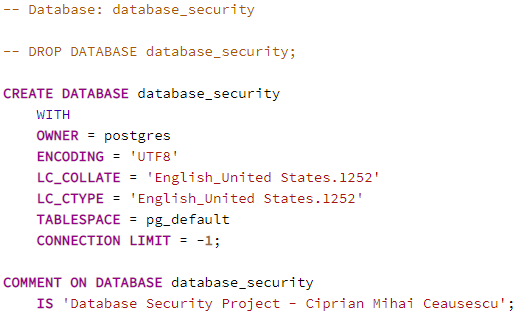
\includegraphics[scale=1]{1}
\caption{Database and tables - Database}
\end{figure}
\begin{figure}
\centering
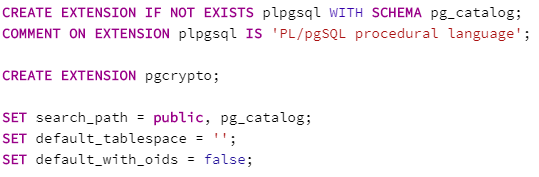
\includegraphics[scale=1]{2}
\caption{Database and tables - Configurations}
\end{figure}
\begin{figure}
\centering
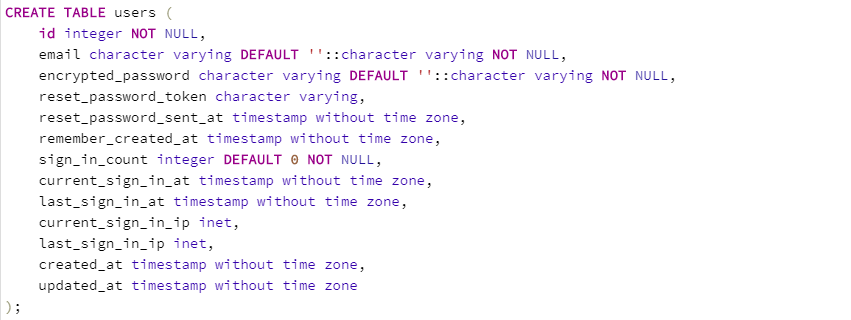
\includegraphics[scale=0.8]{3}
\caption{Database and tables - Users}
\end{figure}
\begin{figure}
\centering
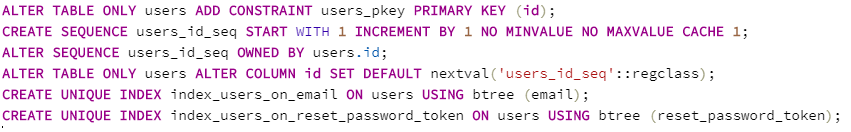
\includegraphics[scale=0.8]{3_1}
\caption{Database and tables - Users}
\end{figure}
\begin{figure}
\centering
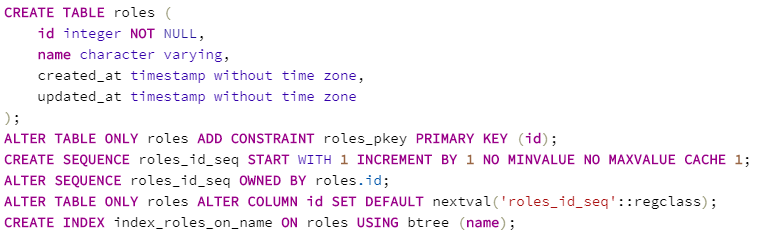
\includegraphics[scale=0.8]{4}
\caption{Database and tables - Roles}
\end{figure}
\begin{figure}
\centering
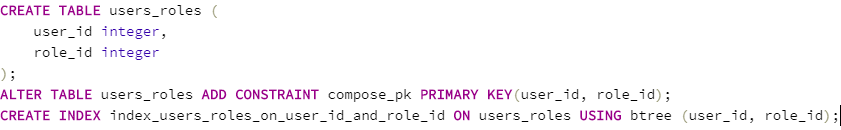
\includegraphics[scale=0.8]{5}
\caption{Database and tables - Users Roles}
\end{figure}
\begin{figure}
\centering
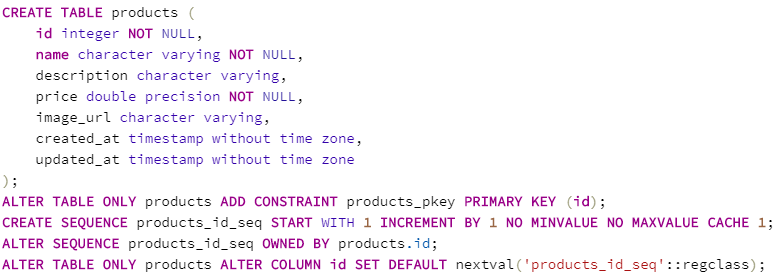
\includegraphics[scale=0.8]{6}
\caption{Database and tables - Products}
\end{figure}
\begin{figure}
\centering
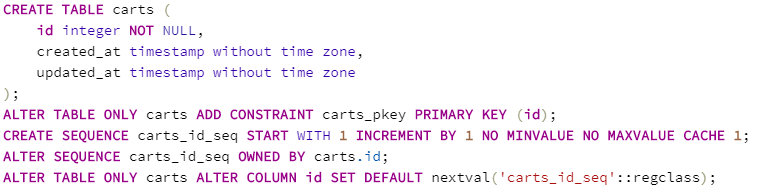
\includegraphics[scale=0.8]{7}
\caption{Database and tables - Carts}
\end{figure}
\begin{figure}
\centering
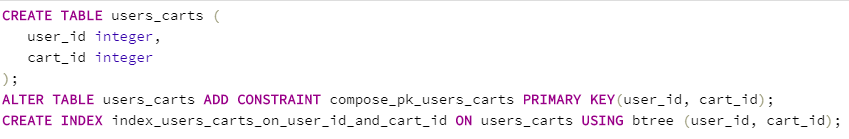
\includegraphics[scale=0.8]{8}
\caption{Database and tables - Users Carts}
\end{figure}
\begin{figure}
\centering
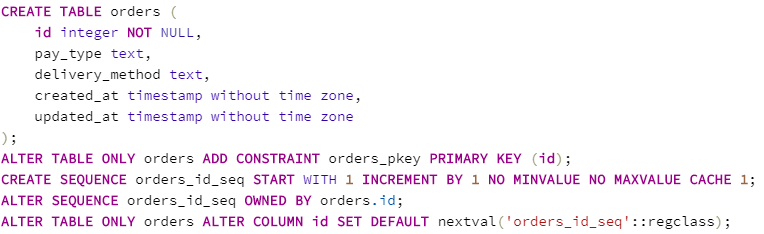
\includegraphics[scale=0.8]{9}
\caption{Database and tables - Orders}
\end{figure}
\begin{figure}
\centering
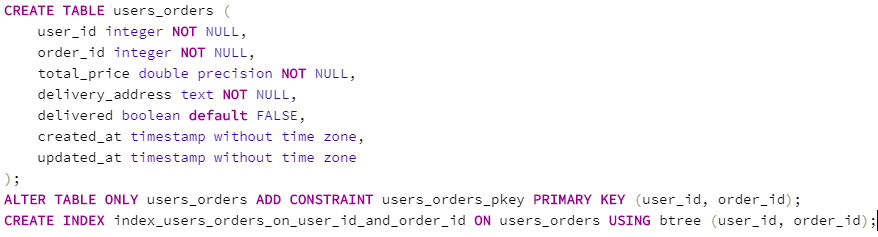
\includegraphics[scale=0.8]{10}
\caption{Database and tables - Users Orders}
\end{figure}
\begin{figure}
\centering
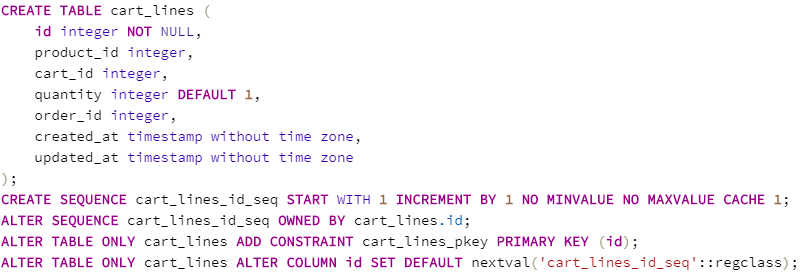
\includegraphics[scale=0.8]{11}
\caption{Database and tables - Cart Lines}
\end{figure}
\begin{figure}
\centering
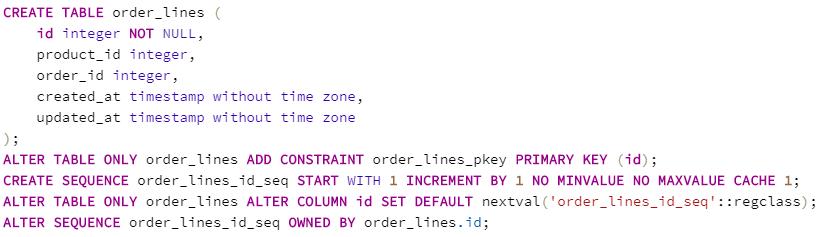
\includegraphics[scale=0.8]{12}
\caption{Database and tables - Order Lines}
\end{figure}
\begin{figure}
\centering
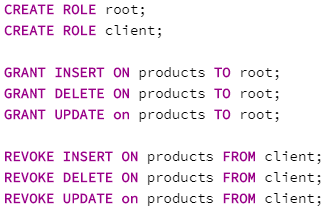
\includegraphics[scale=1]{13}
\caption{Database and tables - Create roles on database}
\end{figure}
\begin{figure}
\centering
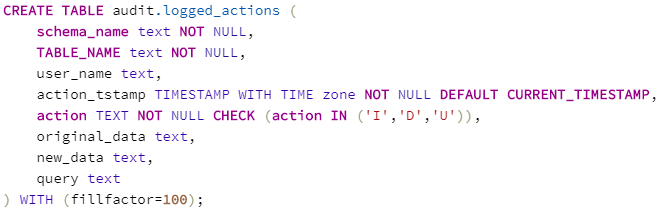
\includegraphics[scale=0.8]{14}
\caption{Database and tables - Logged Actions}
\end{figure}
\begin{figure}
\centering
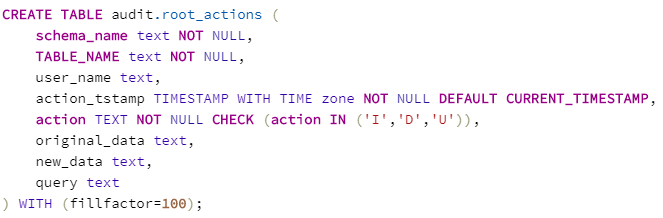
\includegraphics[scale=0.8]{15}
\caption{Database and tables - Root Actions}
\end{figure}
%----------------------------------------------------------------------------------------
%	Functions
%----------------------------------------------------------------------------------------
\begin{figure}
\centering
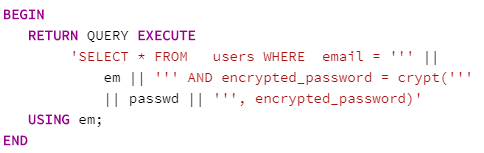
\includegraphics[scale=1]{f1}
\caption{Functions - Login vulnerable}
\end{figure}
\begin{figure}
\centering
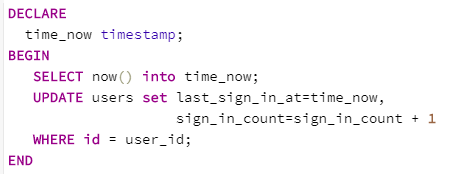
\includegraphics[scale=1]{f2}
\caption{Functions - Audit login}
\end{figure} 
\begin{figure}
\centering
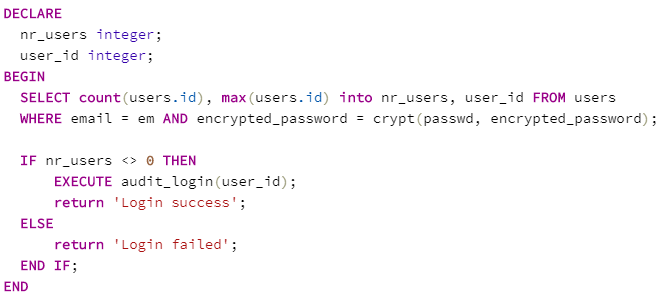
\includegraphics[scale=1]{f3}
\caption{Functions - Login safe}
\end{figure}
\begin{figure}
\centering
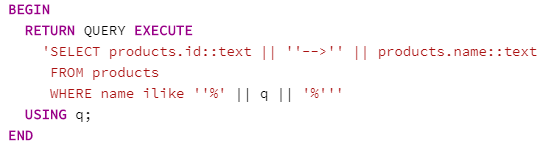
\includegraphics[scale=1]{f4}
\caption{Functions - Search product - vulnerable}
\end{figure}
\begin{figure}
\centering
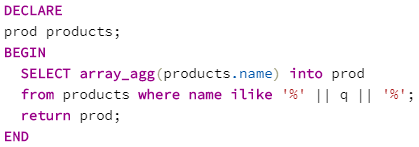
\includegraphics[scale=1]{f5}
\caption{Functions - Search product - safe}
\end{figure}
\begin{figure}
\centering
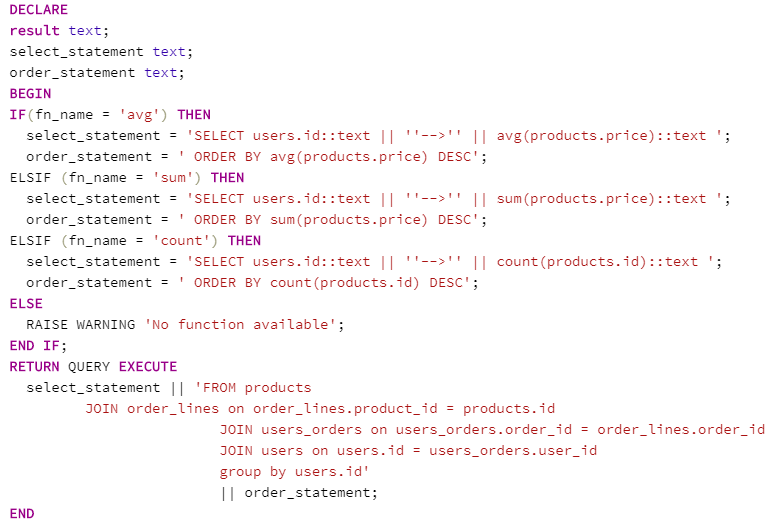
\includegraphics[scale=0.8]{f6}
\caption{Functions - Apply function}
\end{figure}
\begin{figure}
\centering
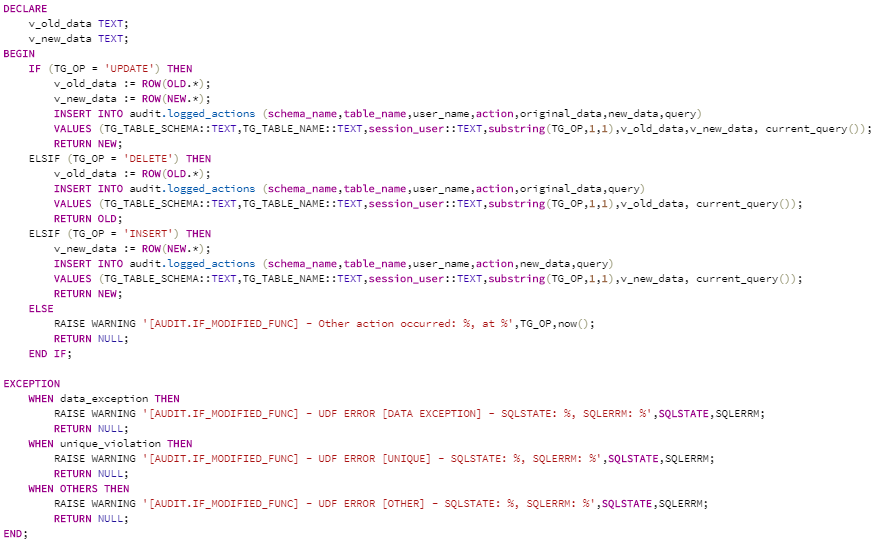
\includegraphics[scale=0.8]{f7}
\caption{Functions - Audit - check if data is modified}
\end{figure}
\begin{figure}
\centering
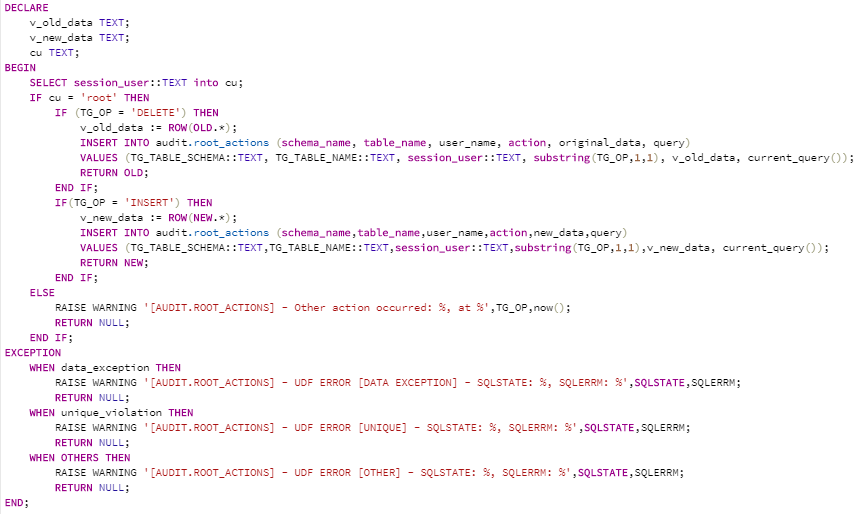
\includegraphics[scale=0.8]{f8}
\caption{Functions - Audit - check if root user made an action}
\end{figure}
%----------------------------------------------------------------------------------------
%	Data
%----------------------------------------------------------------------------------------
\begin{figure}
\centering
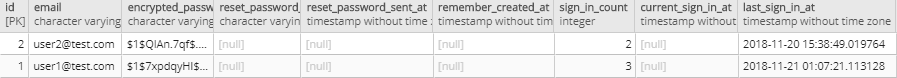
\includegraphics[scale=0.7]{d1}
\caption{Data - Users}
\end{figure}
\begin{figure}
\centering
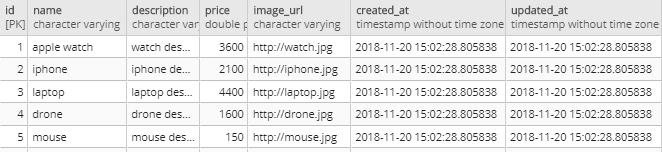
\includegraphics[scale=0.8]{d2}
\caption{Data - Products}
\end{figure}
\begin{figure}
\centering
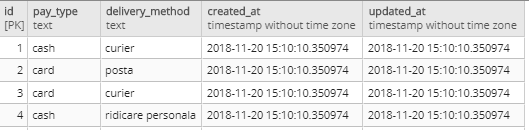
\includegraphics[scale=1]{d3}
\caption{Data - Orders}
\end{figure}
\begin{figure}
\centering
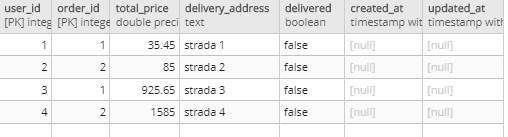
\includegraphics[scale=1]{d4}
\caption{Data - User Orders}
\end{figure}
\begin{figure}
\centering
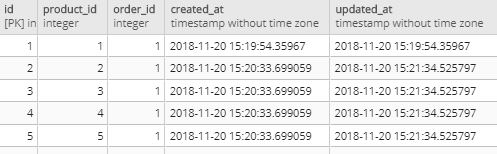
\includegraphics[scale=1]{d5}
\caption{Data - Order Lines}
\end{figure}
\begin{figure}
\centering
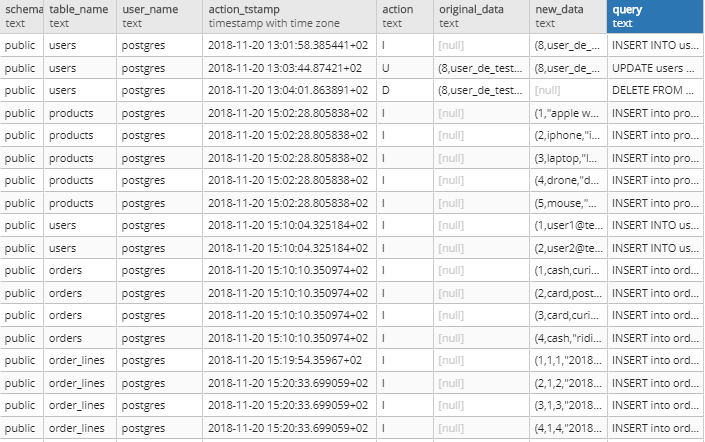
\includegraphics[scale=0.9]{d6}
\caption{Data - Logged Actions}
\end{figure}
%----------------------------------------------------------------------------------------
%	Experimental results
%----------------------------------------------------------------------------------------
\begin{figure}
\centering
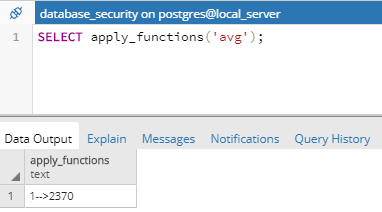
\includegraphics[scale=1]{r1}
\caption{Experimental results - Apply function - avg}
\end{figure}
\begin{figure}
\centering
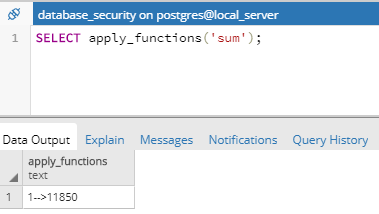
\includegraphics[scale=1]{r2}
\caption{Experimental results - Apply function - sum}
\end{figure}
\begin{figure}
\centering
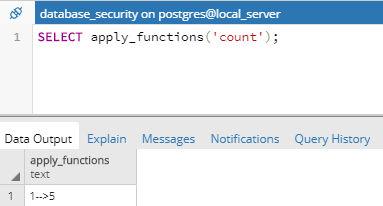
\includegraphics[scale=1]{r3}
\caption{Experimental results - Apply function - count}
\end{figure}
\begin{figure}
\centering
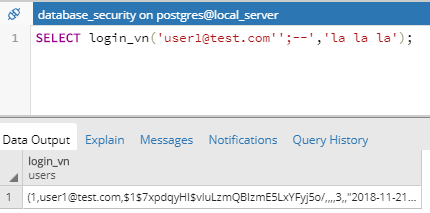
\includegraphics[scale=1]{r4}
\caption{Experimental results - SQL INJECTION TESTS - Gain access without password}
\end{figure}
\begin{figure}
\centering
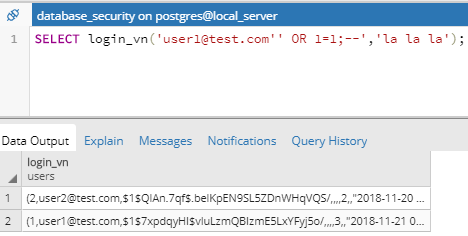
\includegraphics[scale=1]{r5}
\caption{Experimental results - SQL INJECTION TESTS - Dump all users}
\end{figure}
\begin{figure}
\centering
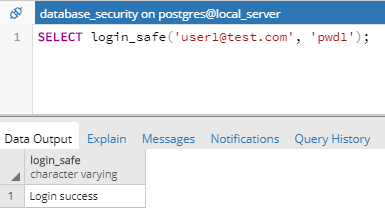
\includegraphics[scale=1]{r6}
\caption{Experimental results - SQL INJECTION TESTS - Login secure - succes}
\end{figure}
\begin{figure}
\centering
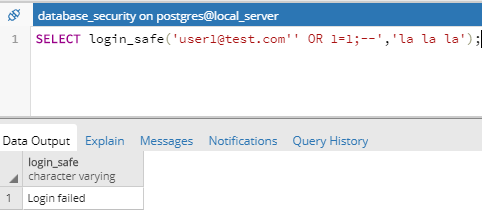
\includegraphics[scale=1]{r7}
\caption{Experimental results - SQL INJECTION TESTS - Login secure - failed}
\end{figure}
\begin{figure}
\centering
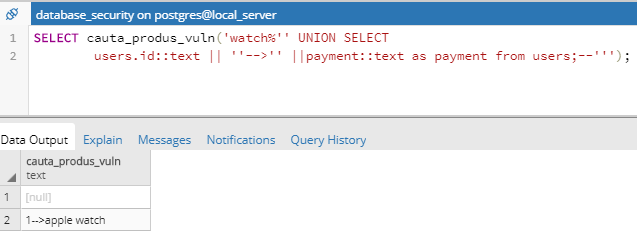
\includegraphics[scale=1]{r8}
\caption{Experimental results - Search products - vulnerable}
\end{figure}
\end{document}
